
% This LaTeX was auto-generated from MATLAB code.
% To make changes, update the MATLAB code and republish this document.











    
    \begin{DoxyCode}
clear
% compile the model
[exdir,~,~]=fileparts(which('example_model_4.m'));
amiwrap('model_example_4','example_model_4_syms',exdir)

num = xlsread(fullfile(exdir,'pnas_data_original.xls'));

t = num(:,1);

D.Y = num(:,[2,4,6]);
D.Sigma_Y = NaN(size(D.Y));


kappa = [1.4,0.45];

xi =  [0.595102743982229
    2.99999999999997
    -0.948930681736172
    -0.00751433662124028
    0
    -2.78593598707493
    -0.256066441623149
    -0.07511250551843
    -0.411247187909784
    -4.99999999959546
    -0.735327875726678
    -0.64146041506584
    -0.107897525629158
    0.0272647740863191
    -0.5
    0
    -0.5];

options.sensi = 0;
sol = simulate_model_example_4(t,xi,kappa,D,options);

figure
for iy = 1:3
    subplot(2,2,iy)
    plot(t,D.Y(:,iy),'rx')
    hold on
    plot(t,sol.y(:,iy),'.-')
    xlim([0,60])
    xlabel('t')
    switch(iy)
        case 1
            ylabel('pStat')
        case 2
            ylabel('tStat')
        case 3
            ylabel('pEpoR')
    end
    ylim([0,1.2])
end
set(gcf,'Position',[100 300 1200 500])

% generate new
xi_rand = xi + 0.1;
options.sensi = 1;
options.sensi_meth = 'adjoint';
sol = simulate_model_example_4(t,xi_rand,kappa,D,options);

options.sensi = 0;
eps = 1e-4;
fd_grad = NaN(length(xi),1);
for ip = 1:length(xi)
    xip = xi_rand;
    xip(ip) = xip(ip) + eps;
    psol = simulate_model_example_4(t,xip,kappa,D,options);
    fd_grad(ip) = (psol.llh-sol.llh)/eps;
end

figure
scatter(abs(sol.sllh),abs(fd_grad))
set(gca,'XScale','log')
set(gca,'YScale','log')
xlim([1e-2,1e2])
ylim([1e-2,1e2])
box on
hold on
axis square
plot([1e-2,1e2],[1e-2,1e2],'k:')
xlabel('adjoint sensitivity absolute value of gradient element')
ylabel('finite difference absolute value of gradient element')
set(gcf,'Position',[100 300 1200 500])
\end{DoxyCode}

         \begin{DoxyCode}Generating model struct ...
Parsing model struct ...
Generating C code ...
headers | wrapfunctions | 
Compiling mex file ...
Building with 'Xcode with Clang'.
MEX completed successfully.
\end{DoxyCode} 
    
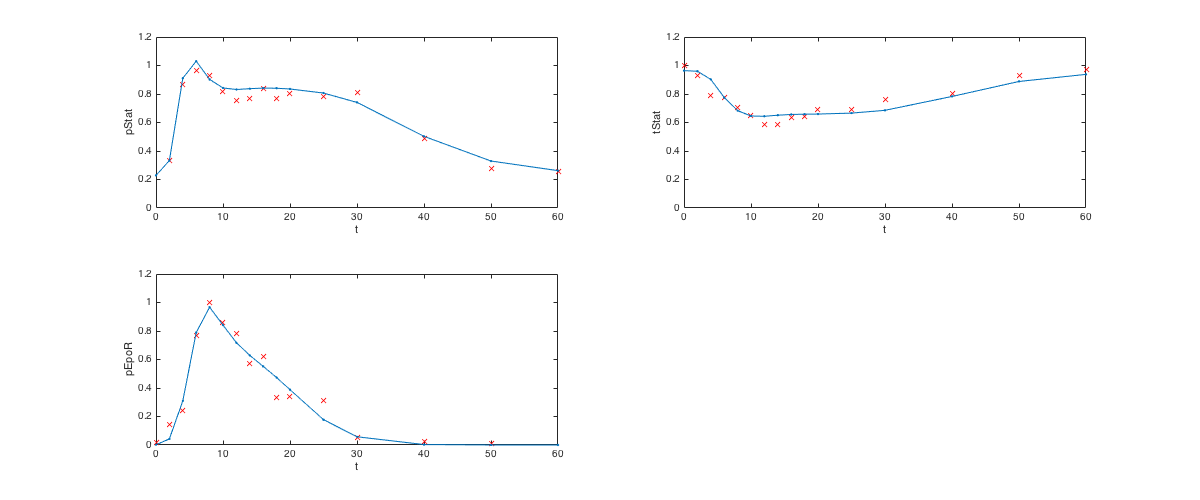
\includegraphics [width=4in]{../../examples/example_4/html/example_model_4_01.png}

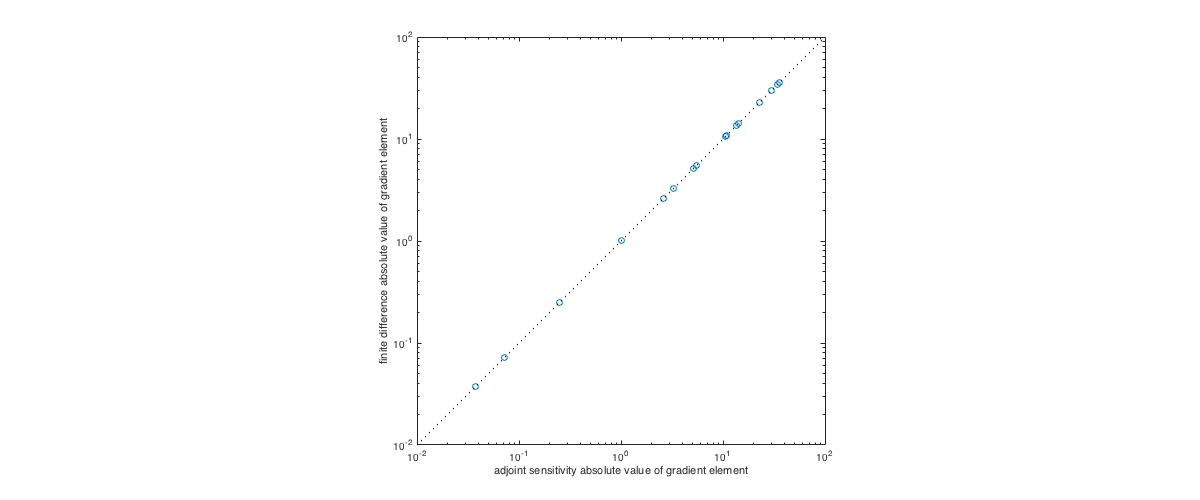
\includegraphics [width=4in]{../../examples/example_4/html/example_model_4_02.png}




    